\section{System Design}
\label{sec:design}

\subsection{System components}
As we stated before, the backlight scaling technique involves three
stages for 1) generating luminance histogram, 2) determining backlight
levels and 3) compensating the pixel luminance. Thence these stages are
decoupled into three independent modules in our system respectively:
{\bf scanning module}, {\bf adjustment module } and {\bf rendering
  module }. The organization of these three modules are shown in the
Figure~\ref{fig:design}.

\begin{figure}[t]
  \begin{center}
  \label{fig:design}
  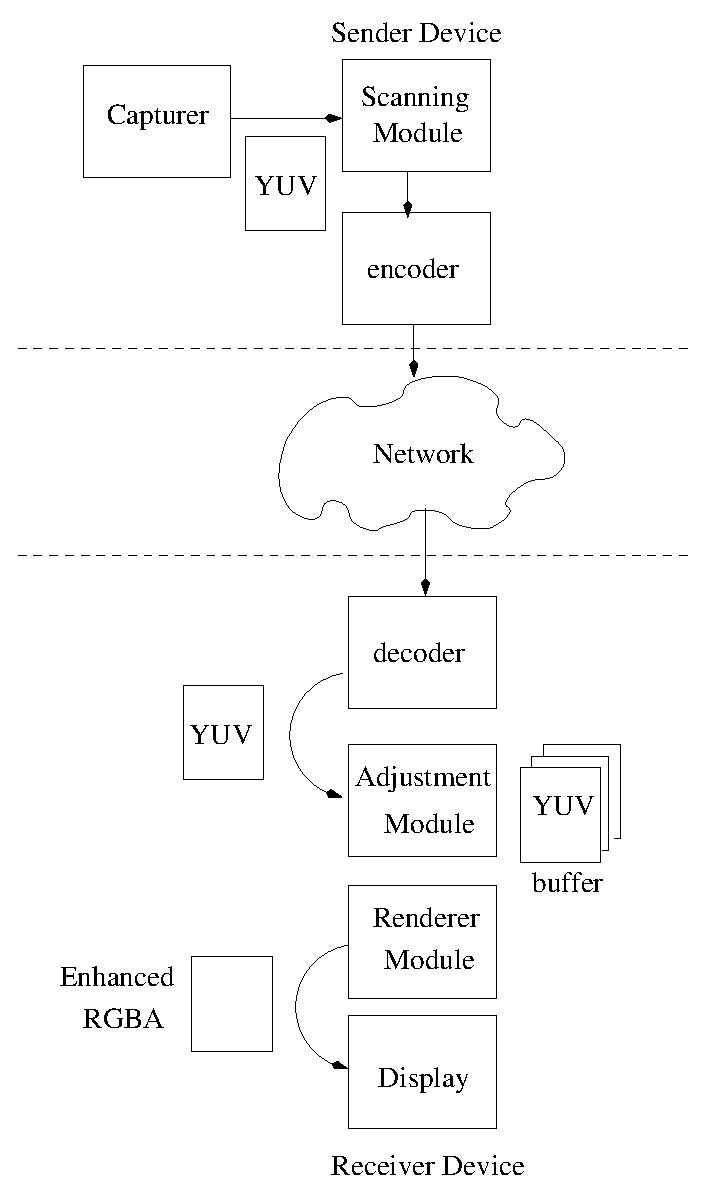
\includegraphics[scale=.5]{./figures/design.eps}
  \caption{System Design}
  \end{center}
\end{figure}


{\bf Scanning module } is the component extracting the pixel luminance
information. In the real-time communication, the frames are generated
by the capturer, which is usually a physical camera. There is no way
to access the video content in advance. So the scanning module is
necessary to generate the luminance histogram for later determination
stage and compensation stage. Other than the Video On Demand (VOD),
the RTC session involves $N \ge 2$ participants. The eventually
rendered image is composed by all received frames (including that from
the receiver itself). The scanning module is better installed at the
sender side, so that each generated frame will be scanned only
once. However, this brings another problem that how to transmit this
information to the receivers. Building another channel introduces
additional overhead and extra effort must be made to synchronize the
frames and the luminance information. Either of them may not arrive
the receiver on time. For more efficiency on the luminance information
transmission, we choose to encode this information with the frame
data. In our scheme, the bottom cornors are the best candidates. This
position either is covered by other frames, or is negligible when the
frame is resized too small. By doing this, we still risk losing the
luminance information in the encoding process and network
transmission. So we duplicate this information and set them at the
positions known by both ends. The receiver side extracts the
information and use the value elected from the majority, and then
passes the value to next adjustment module for backlight scaling.

{\bf Adjustment module} is located at the receiver side. This module
tries to find the apprapriate backlight levels from the luminance
information. In the VOD, global luminance information is required to
prevent the flickering effects, which is caused by scaling the
backlight in great variation too frequently. But the latency is less
tolerant in the real-time communication, so buffering amounts of frames
for the purpose of waiting for enough luminance information to get
optimal backlight levels is not practical. We proposed to use a greedy
algorithm in the determination stage. This algorithm determines
current backlight level only based on the last one. So little latency
is likely to be introduced into the system. After this, adjusted
backlight levels are sent to the rendering module for pixel
compensation and backlight scaling. 

{\bf Rendering module} strengthens the original rendering function by
adding pixel compensation and backlight scaling. The GPU is used to
enhance the pixel luminance. Since the GPU has been enabled for
resizing, composing the received frames and performing RGB-YUV
conversion, trivial power consumption is introduced by the adding the
pixel compensation task. This module also scales the backlight levels
making the images on the screen perceived no distorion from the
original version. 

\subsection{Backlight determination algorithms}
Before the $t$'th frame is rendered on the screen, the corresponding
backlight level $b_t$ must be determined. An intuitive way is to set the
$b_t$ by the maximum luminance $Y_{t}^{max}$ to achieve the most power
savings. However, this may undermine the user experience by
introducing flickering effects and also the hardware can not response
the backlight instructions promptly. To find the lowest backlight
levels without viodlating the user experience constraint and the
hardware constraint, some dyanamic programming algorithms are
proposed. 


%% The basic idea of luminance compensation is when the backlight is
%% dimmed, the luminance of frame pixels are enhanced. Thence the power
%% savings are achieved while no observable distortion exists. In next
%% sections, we denote the $t = 1, 2, ...$ as the frame index in a live
%% streaming. And the $Y_{t}^{max} \in [0, 255]$ is the max luminance of
%% frame $t$. The $b_{t} \in [0, 1]$ stands for the target backlight
%% level when the $t$th frame is rendering.

\subsubsection{Optimal solution}
The dynmamic programming solution is trying to find the optimal
backlight levels across the video playback without violating the
constraints mentioned before. This algorithm is represented by the
recursion equation~\ref{eq:dp}:

\begin{equation}
  \label{eq:dp}
B(t,b) = \min_{t',b'}(b \times (t - t') + B(t', b')) 
\end{equation}
where $B(t, b)$ stands for the minimum summation of backlight levels
from the beginning of the video to the $t$'th frame while the
backlight level of the $t$'th frame is scaled to $b$. The $t'$ is the
frame index where the last backlight level is determined and the $b'$
is the last determined backlight level. When this algorithm is seeking
the optimal solution, it must comform to the following constraints:

%% \[
%%  \left \{
%% \begin{array}{l}
%%   \[\label{eq:hah} a = 10 \] \\
%%   b\ \text{or}\ b' \ge Y^{max} / 255 \smallskip \\
%%   t' \in [\ t - l_{max},\ t - l_{min}] \smallskip \\
%% \end{array}
%%   \right.
%% \]

\begin{equation}
  \label{eq:distort}
  b \ge \frac{Y^{max}}{255}
\end{equation}
\begin{equation}
  \label{eq:userexp}
  b \in [\ b' \times ( 1 - \Delta_b ),\ b' \times ( 1 +
    \Delta_b)]
\end{equation}
\begin{equation}
  \label{eq:hardware}
  t' \in [\ t - l_{max},\ t - l_{min}] 
\end{equation}


The equation~\ref{eq:distort} represents the distortion constraint,
where the $b$ follows the $Y^{max}$ of the corresponding frame and
so does the $b'$. Otherwise the distortion will be introduced. The
user experience constraint is quantified as the relationship between
the $b$ and the $b'$ in the euquation~\ref{eq:userexp}. The neighboring
$b$ and $b'$ is not allowed to differentiate too much to prevent the
flickering effects. We define the $\Delta_b$ as the upperbound of the
luminance variation of the continuous frames. The last equation~\ref{eq:hardware}
means the hardware constraint. For at least $l_{min}$ frames, the
backlight levels will stay at the same value. The $l_{max}$ is imposed
to reduce candidates of $t'$ in each recursion step. The result will
be the global optimal if $l_{max}$ is the total frame number of the
playing video. 

%% Although the ideal case is the pixels of the $t$th frame are enhanced by
%% $(255 - Y_{t}^{max})$, so that the $b_{t}$ can be scaled to
%% $\frac{Y_{t}^{max}}{255}$, which is the minimum possible value, 
%% without losing any observable fidelity. However, if we do this
%% practically, two negative phenomenons are found:
%% \begin{itemize}
%%   \item{The {\it flickering} is found as the screen backlight varies
%%     dramatically.}
%%   \item{On devices, The backlight scale can't react in real-time
%%     manner. The hardware response the scaling directive in a short
%%     delay.}
%% \end{itemize}
%% Both of the facts should be taken into account when we scale the
%% backlight. Since it is so, we quantify the next three
%% constraints. With the $\Delta_{b}$, which stands for the max allowed
%% backlight difference in one adjustment operation, we have
%% $b_{t+1} \in [b_t \times (1 - \Delta_t), b_t \times (1 + \Delta_t)]$.  And another
%% constraint is the $l_{min}$, which stands for the frame number which
%% must keep same backlight level. The last one is that $b_{t} <
%% \frac{Y_{t}^{max}}{255}$, keeping the backlight level in its $[0,1]$
%% range.  its . we will get the Dynamic Programming solution from this
%% recurrence:

%% More explanations later...

\subsubsection{Greedy solution}
\label{sec:greedy}
Certainly the dynamic programming technique can provide the optimal
backlight levels without violating the adjustment constraints. However
it is impractical to adjust the backlight levels in the RTC session in
this way. The dynamic programming must hold amounts of frames before
it determines the bakclight levels, and this leads to significant
latency between the sender and the receiver. In our greedy solution,
we make attempt to relax the constraints in the dyanmic
programming--our scheme ignores the distortion constraint in
euqation~\ref{eq:distort}. We expect our scheme won't leads to amounts
of distortion based upon the intuition that few scene switches are
likely to be found during the RTC session. 


%% The DP algorithm certainly can offer us the best solution on adjusting
%% the backlight over the frames. And the greedy version can also help
%% achieve the similar effect. Except that we have to render some frames
%% in distortion without violating the constraints.

\begin{algorithm}
  \caption{the greedy algorithm}
  \label{alg:greedy}
  \begin{algorithmic}[1]
    \LineComment{On input $(t, Y_{t}^{max}, b', t')$, where $b'$
      is the last adjusted backlight level and the $t'$ is the
      corresponding frame index, we generate the $b_{t}$, the
      backlight level of the $t$'th frame. }
    \\
    \If {$t = 1$}
      \State $b' \gets Y_{t}^{max} / 255$
      \State $t' \gets t$
      \State $b_t \gets b'$
      \Return $b_t$
    \EndIf
      \\
    \If {$t - t' < l_{min}$}
      \Return $b'$
    \EndIf
    \\

    \State $b_{t} \gets Y_{t}^{max} / 255$
    \If {$b_{t} < b' \times (1 - \Delta_{b})$}
      \State $b' \gets b' \times (1 - \Delta_{b})$
    \ElsIf {$b_{t} > b' \times ( 1 + \Delta_b)$}
      \State $b' \gets b' + (1 + \Delta_{b})$
    \Else
      \State $b' \gets b_t$
    \EndIf
    \\
    \State $b_{t} \gets b'$\\
    \State $t' \gets t$
    \Return $b_{t}$
  \end{algorithmic}
  
\end{algorithm}


Our greedy version adjustment method is shown in the
algorithm~\ref{alg:greedy}. The backlight level of $t$'th frame, the
$b_t$, only depends on the last adjustd backlight level $b'$, its
index $t'$ and the maximum luminance of current frame $Y_t^{max}$. In
the adjustment, the $b_t$ still comform to the constraints represented
in equation~\ref{eq:userexp} and \ref{eq:hardware}. The distortion may
occur is the $Y_t^{max}$ and $b_t$ can not satisfy the
equation~\ref{eq:distort}. With the assumption of that there is no
frequent scene switches in the RTC, we expect such distortion will be
corrected gradually in next adjustment operations.



%% we input the luminance
%% $Y_{t}^{max}$ of $t$th frame and get the target backlight level
%% $b_{t}$ for future adjustment. Then we can scale the backlight when
%% the corresponding frame is shown on the display. However, the distortion
%% may occur if the $t$th frame has the max luminance $Y_t^{max}/255 >
%% b_{old} + \Delta_b$.



\section{implementation}
\label{sec:implementation}

We built our system base on AppRTC, which is part of the project
chromium. This Android app links to libjingle.so, which is the WebRTC
support library of Chrome browser. The scanning module and adjustment
module resides inside the libjingle.so and Rendering module is part of
the Android app.


%% \begin{itemize}
%%   \item
%%     {
%%       Local DP.
%%     }
%%   \item
%%     {

%%       right-bottom is not significant

%%       set the pixels around the frame. if it doesn't match, select the
%%       most candidate or the last one. 
%%     }
%%   \item
%%     {
%%       skipping some frames.
%%     }
%% \end{itemize}

%% It's not so effective if we process per frame at the receiving end and


%% This is not advisable in
%% the real-time communication since latency is inacceptable in 
%% This
%% component is used to accept frames decoded from the decoder. 
%% This component
%% can buffer the frames, fetch out luminance information and then
%% perform the adjustment. The resulting values of brightness are sent to
%% the next module for following rendering. The module locates the
%% receiver side to avoid built another channel over the network for
%% passing the adjusted brightness values. The strategy used to adjust
%% brightness is chosen between the DP and Greedy mentioned before.



%% In one real-time communication session of $N$
%% participants, each frame rendered on the screen is composed of $N$
%% received frames. For the purpose of scanning every generated frame
%% only once, this module is put at the sender side, just between the
%% encoder and capturer, which is usually a physical camera. The scanning
%% module accepted all frames captured by the capturer in YUV
%% format. Before these frames are sent to the encoder, the scanning
%% module find out the maximum luminance in this frame and write this
%% value at the lower cornors. Since this information may lose in future
%% encoding/decoding and network transmission, we write redundant values
%% into the frame.


%% In later stage, the maximum luminance In the real-time communication, there is no way to
%% collect such information in advance. This scanning operation has to be
%% performed with the frame rendering simultaneously. As a result, if
%% the videos must satisfy some quality requirement in fps, the scanning
%% moduel has only limited time to generate the luminance histogram. For
%% example, a conversation streaming of $30$ fps can provide at most ~$33$
%% ms for the each frame being scanned. Then if considering the latency of
%% accessing main memory is the order of $100$ ns, then an estimation of $92$ ms is
%% required to find 

%% Practically whether such task can meet the
%% rendering deadline -- at most $33$ milliseconds is permitted to scan
%% one frame in a video of $30$ fps -- depends on the quality of the
%% video. Considering the latency of accessing main memory is the order
%% of $100$ ns, ~$92$ ms is required to generate the luminance
%% histogram of a $1280$x$720$ image. This operation definately degrades
%% this video streaming by decreacing the fps. 

%% (/ (* 100 (* 1280 720)) 1000000.0)
%% (/ (* 640 480 100) 1000000.0)
%% (/ 1000.0 92)



%% The {\bf scanning module} is responsible of extracting pixels
%% luminance information of frames. If we run this task on the CPU, we
%% may miss the deadline of rendering the frames in a higher fps
%% manner. considering the latency of accessing main memory is $100$ ns,
%% ~$92$ ms is required to scan a $1280$x$720$ frame. And ~$30$ ms for a
%% lower quality frame of $640$x$480$. This histogram generation task is
%% actually best fit the GPU feature, which is highly parallel
%% and no interactive operations. The GPU performance is so good 

%% This makes the fps hardly
%% exceed $10$ in a high quality conversation session. If we are
%% satisfied with the upper bound of $15$ fps, and a low-quality image of
%% $640$x$480$. we can use the CPU to do this work, otherwise, we have
%% launch the GPU to get the historgram data. However the data calculated
%% from GPU must be copied between GPU memory and CPU memory. So this is
%% not so effecient if with low quality image. 

%% 1) location 2) 

%% The system logically contains three components. The first one is the
%% {\bf Scanning module}, which is responsible of scanning YUV frames for
%% liminance information.  Unlike the case of playing VOD or local
%% Videos, real-time communication is featured both frame generation and
%% frame rendering. Hence this module can either locate at sender side,
%% before the encoder, or receiver side, after the decoder. The sender is
%% an evidently better option. If the Scanning module sits at the
%% receiver side, thinking of the scenario where $N$ users are involved
%% in a video conference, each client have to scan $N$x frames. To also
%% reduce the frame number to $1$ per frame at the receiver side, the
%% system can only scan the composed frame at rendering time. This makes
%% the time too stringent and the DP is not a option for adjust backlight
%% any more. Further, the scaling operation always got behind with
%% rendering operation due the hardware constraint. After scanning, the
%% max luminance information is hidden inside corresponding frame. To
%% avoid packet loss in network transfer, we set the max luminance value
%% at all four corners. When these values are fetch out, the most
%% equivalent value is elected as the max luminance of this frame.


%% We intend to use CPU other than GPU to scan the raw frame. 1)
%% practically the resolution and fps in real-time communication
%% streaming is usually lower than other stream case. CPU is completely
%% capable of doing this in time. 2) The GPGPU and technique has little
%% threads priority mechanism, especially on the mobile platform. While
%% another GPU-related task(YUV conversion and frame composition) has
%% obviously higher priority is most likely to be occupied. 


%% adjust the space of pixels to emluminance and also notice the system
%% to scale its backlight. What I need mention is that if we have to
%% perform the DP, we have to equip a queue of size greater than
%% $1$. two reason we prefer the Greedy version.
%% 1) The network bandwidth throttle the size of queue. make it hardly
%% achieve global optimization in backlight scale. 
%% 2) In the case of real-time communication, the variation of scenarios
%% is little. We hardly meet the case of luminance raise or drop
%% abruptly.

%% The third component is the {\bf Rendering Module}. For the system which
%% already has the function of conversion between YUV and RGBA frames,
%% plug the function of lightening pixels just before this
%% conversion. Also this module is responsible of sending the backlight
%% scaling requests to OS at the appropriate time point so that display
%% can be correctly compensated. 
%%  of frame $t$ by  of When the frames are composed and
%% before convert to RGBA format in shader. we increase the Y component. 

%% unlike the streaming or local video play case, the real-time
%% communication need compose several frames together(e.g, in
%% peer-to-peer case, typically the opponent's head occupy the most
%% display and the picture of the users lay at the bottom of display).
%% we must efficiently compose these pictures together in using GPU
%% without dropping the fps. Finally, we don't need risk the high power
%% consumption difference between GPU on-and-off. We only afford the
%% extra computation power consumption.


